
\subsection*{3.1 Plane Geometry}
Plane geometry deals with shapes, lines, and angles in two-dimensional space. Understanding the properties of various geometric figures is fundamental to solving problems in geometry.

\textbf{Key Concepts:}

\paragraph{Triangle and its Properties:} A triangle is a three-sided polygon with three angles. The sum of the interior angles of a triangle is always $180^\circ$. Triangles can be classified based on their sides (scalene, isosceles, equilateral) or angles (acute, right, obtuse). The exterior angle of a triangle is equal to the sum of the two opposite interior angles.
\begin{center}
	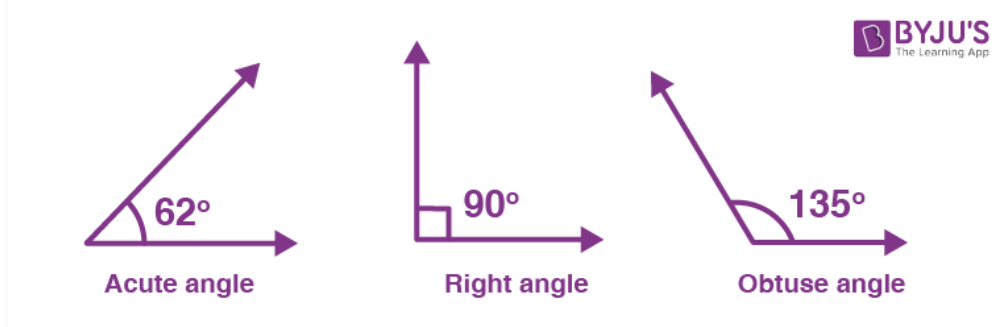
\includegraphics[width=0.6\textwidth]{3.10.png}
\end{center}


\paragraph{Pythagoras Theorem:} In a right-angled triangle, the square of the hypotenuse (the side opposite the right angle) is equal to the sum of the squares of the other two sides. Mathematically:
\[
c^2 = a^2 + b^2,
\]
where $c$ is the hypotenuse, and $a$ and $b$ are the other two sides.

\paragraph{Quadrilaterals and Their Properties:} A quadrilateral is a four-sided polygon with four angles. Common types include squares, rectangles, parallelograms, trapeziums, and rhombuses. 
The sum of the interior angles of a quadrilateral is $360^\circ$. Specific properties include:
\begin{itemize}
	\item Opposite sides of a rectangle and parallelogram are equal.
	\item Diagonals of a square bisect each other at right angles.
	\item A trapezium has one pair of parallel sides.
\end{itemize}

\paragraph{Inscribed Triangles and Polygons:} An inscribed polygon is one whose vertices all lie on a single circle, called the circumcircle. The center of this circle is called the circumcenter, and the radius is the circumradius. For inscribed triangles, the angle subtended by a diameter at the circumference is always a right angle.

\paragraph{Internal and External Angles of Triangles and Polygons:} The sum of the internal angles of a polygon with $n$ sides is:
\[
(n-2) \times 180^\circ.
\]
The sum of the external angles of any polygon is always $360^\circ$, making each exterior angle equal to 
\[
\frac{360^\circ}{n}.
\]

\paragraph{Polygons and Their Properties:} Polygons are closed figures with three or more sides. Regular polygons have equal sides and angles. Examples include pentagons, hexagons, and octagons. The measure of each internal angle of a regular polygon with $n$ sides is:
\[
\frac{(n-2) \times 180^\circ}{n}.
\]

\textbf{Examples:}

\begin{flushleft}
	\textbf{Example 1: Calculate the hypotenuse of a right triangle with sides 3 cm and 4 cm.}
	
	\vspace{0.5cm}
	\textbf{Solution:}
	\vspace{0.5cm}
	
	Use Pythagoras theorem:
	\[
	c^2 = a^2 + b^2 = 3^2 + 4^2 = 9 + 16 = 25.
	\]
	\[
	c = \sqrt{25} = 5 \text{ cm}.
	\]
	Therefore, the hypotenuse is 5 cm.
\end{flushleft}

\begin{flushleft}
	\textbf{Example 2: Find the sum of the internal angles of a hexagon.}
	
	\vspace{0.5cm}
	\textbf{Solution:}
	\vspace{0.5cm}
	
	For hexagon n=6.\\
	Use the formula for the sum of internal angles of a polygon:
	\[
	(n-2) \times 180^\circ = (6-2) \times 180^\circ = 4 \times 180^\circ = 720^\circ.
	\]
	Therefore, the sum of the internal angles of a hexagon is $720^\circ$.
\end{flushleft}

\begin{flushleft}
	\textbf{Example 3: A square is inscribed in a circle. Find the radius of the circle if the side of the square is 8 cm.}
	
	\vspace{0.5cm}
	\textbf{Solution:}
	\vspace{0.5cm}
	\begin{center}
		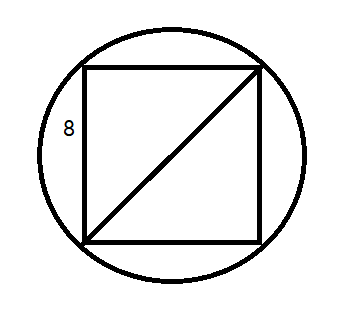
\includegraphics[width=0.6\textwidth]{3.2.png}
		
	\end{center}
	The diagonal of the square is the diameter of the circle. Use the Pythagoras theorem:
	\[
	diagonal^2 = side^2 + side^2 = 8^2 + 8^2 = 64 + 64 = 128.
	\]
	\[
	diagonal = \sqrt{128} = 11.31 \text{ cm}.
	\]
	The radius is half the diagonal:
	\[
	radius = \frac{11.31}{2} = 5.66 \text{ cm}.
	\]
	Therefore, the radius of the circle is 5.66 cm.
\end{flushleft}

\begin{flushleft}
	\textbf{Example 4: Find each internal angle of a regular pentagon.}
	
	\vspace{0.5cm}
	\textbf{Solution:}
	\vspace{0.5cm}
	
	Use the formula for each internal angle of a regular polygon with n=5:
	\[
	\frac{(n-2) \times 180^\circ}{n} = \frac{(5-2) \times 180^\circ}{5} = \frac{3 \times 180^\circ}{5} = \frac{540^\circ}{5} = 108^\circ.
	\]
	Therefore, each internal angle of a regular pentagon is $108^\circ$.
\end{flushleft}
